% #############################################################################
% This is Chapter 2
% !TEX root = ../main.tex
% #############################################################################
% Change the Name of the Chapter i the following line
\fancychapter{Power Availability Forecasting - Background and Related Work}
\cleardoublepage
% The following line allows to ref this chapter
\label{chap:background}

This chapter presents an overview of the fundamental and most commonly used models in \textit{Building Power Consumption and Production Forecasting}, along with a revision of the related work in the field.

Before starting to dissect the history of predictive methodologies, one must consider that \textit{Time Series Forecasting} is an area with numerous applications, and can be applied to several fields of research. Given the high consumption of buildings, as well as its trending behaviour, the prediction of this factor can be the core basis for the development of intelligent systems, capable of optimizing resources to contribute to a more sustainable system overall.


\section{Methodologies\label{a}}

Over the past decades, numerous methods have been created to meet the challenge of predicting the energy behavior of any system, namely buildings and large architectural structures. The increase in the processing capacity of computers and the technological advance, in general, have been contributing to faster solutions, capable of obtaining more accurate results in a shorter time span.

Currently, the approaches used for building energy prediction and/or simulation are roughly categorized as: (1) white-box based approaches, (2) grey-box based approaches, and (3) black-box based approaches \cite{review2017}. White-box methods are based mostly on knowledge about the system. This family of methods requires knowledge of detailed information about the building in question, which makes it possible to obtain good accuracy in the forecasts obtained, but makes the models slow and complex to use. Grey-box methods are known to combine the white-box approach with data regarding the past energetic behaviour of the building, and apply statistical evaluations to predict future energy consumption. Finally, the black-box methods are able to perform an assessment, and produce a forecast of a building's energy consumption, based only on the building's statistical and historical information from the data, discarding the building's specific details (as is done in the other two methods), allowing this last type of methods to produce results with better accuracy and at a much faster pace than the other alternatives. The main disadvantage is that, in order to obtain a really useful and acceptable forecast, there must be a high amount of past data available to train and evaluate the model.

The work developed in this thesis aims to find a solution to the proposed problem through \ac{ML} techniques, which means that the focus of this work and respective research is based on black-box or, from now on, data-driven techniques.

\section{Data-driven forecasting techniques\label{b}}

In 2020 there is a wide range of forecasting methodologies. Since data-driven techniques have been widely used for forecasting energy patterns, we will focus our research on this class of predictive techniques. In Figure \ref{datamodels}, there is a representation of some of the most common models applied in forecasting tasks.

\begin{figure}[h!]
    \centering
    \begin{center}
    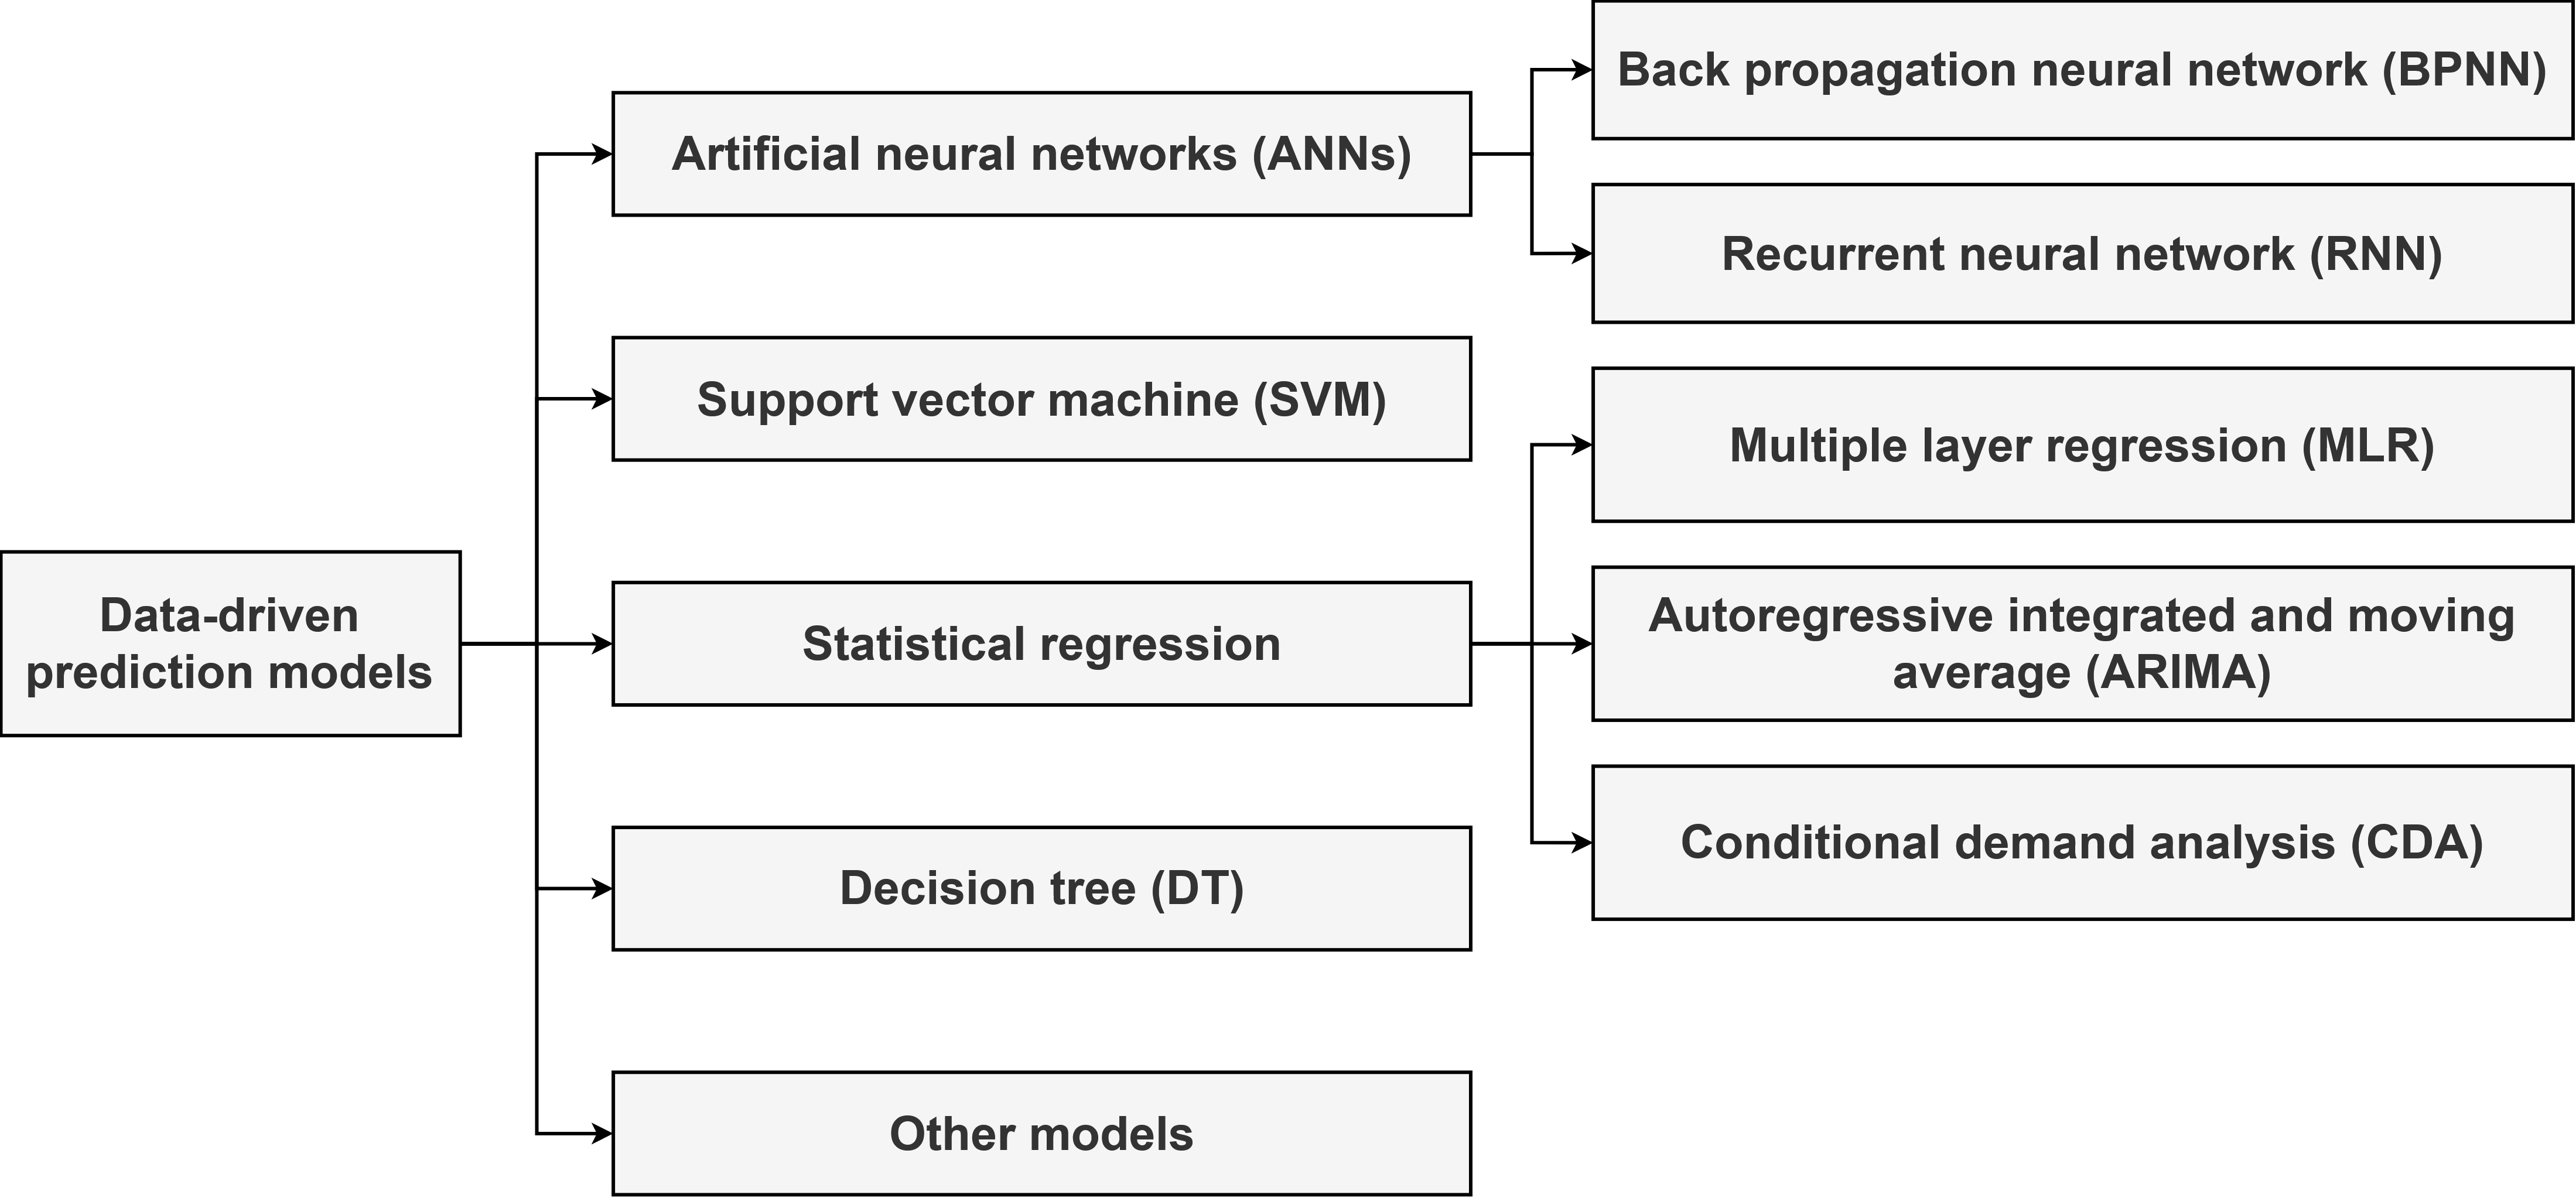
\includegraphics[width=1\textwidth]{Images/data-drive prediction models.png}
    \caption{Different data-driven models for forecasting tasks.}
    \label{datamodels}
    \end{center}
\end{figure}

To better understand how each one of these methodologies work, let us then move on to explain each of the main categories: \acf{ANNs}, \acf{SVMs}, Statistical regression, \acf{DTs}, and other models.


\subsection{Artificial neural networks (ANNs)}

Inspired by human brain architecture, a typical neural network consists of an interconnected group of artificial neurons, and it contains information using a connection list approach to computation \cite{ann1}. The application of this methodology has had enormous success when applied to nonlinear problems. Structurally, \ac{ANNs} consist of a large number of neurons arrayed in different layers, connected with one another via connections \cite{review2017}. In Figure \ref{neuron}, it is possible to observe a representation of the basic computing element of an \acs{ANN}, the neuron. 
The neuron has a unique behavior, since it receives one or multiple inputs $I_i$ from other units or neurons, and each one of these inputs, has a weight $w_i$ associated, which changes its value based on the previous training of the network, in order to adjust the value of the input based on the proposed goal. The architecture of the neuron can be divided into two sections, in which the first adds products of weight coefficients and input signals, and the second section realizes the nonlinear function, called neuron activation function, i.e. $f(.)$. Therefore, the output function of the neuron is given by \cite{ann1}

\begin{equation}
   y = f(\sum_i w_i I_i + bias), 
   \label{tauequation}
\end{equation}

where the $bias$ is specific for each iteration and unit, and $f(.)$ is the activation function. The most common activation function is the sigmoid function \cite{ann1}, give by

\begin{equation}
   f(x) = \frac{1}{1+e^{-x}}.
   \label{fequation}
\end{equation}

This function, presents a s-shape, and is responsible for mapping all the input values to the interval [0, 1], converting the actual value into a value that can be interpreted in probabilistic terms. As the properties of common networks dictate, each neuron can serve as an input from the neuron in a next layer and so on. In Figure \ref{mlp}, it is possible to see a schematic representation of an \acs{ANN}. It can be verified that it presents, as previously mentioned, a layered structure. 

\begin{figure}[h!]
\captionsetup[subfigure]{position=b}
\centering
\subcaptionbox{\label{neuron}}{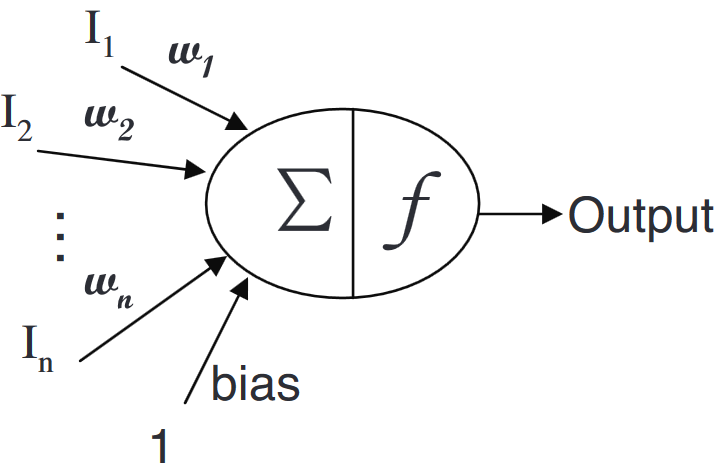
\includegraphics[width=.4\linewidth]{Images/neuron.PNG}}
\hspace{0.05\textwidth}
\subcaptionbox{ \label{mlp}}{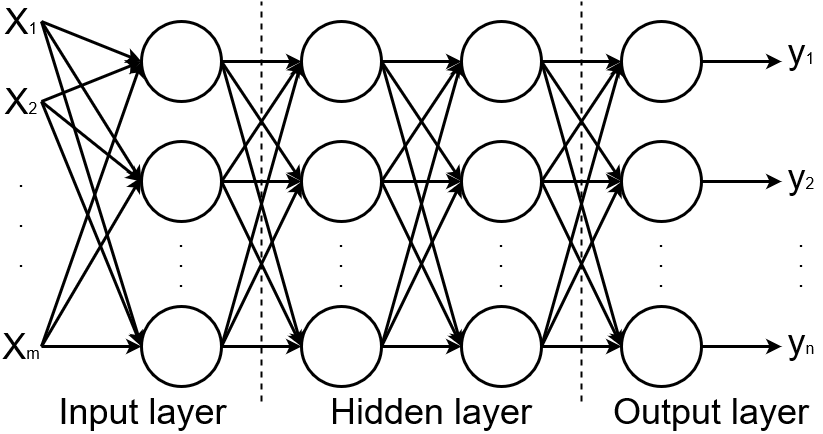
\includegraphics[width=.49\linewidth]{Images/ANN.png}}
\caption{Example of a) a neuron and a b) multi-layer perceptron.}
\end{figure}

The Figure \ref{mlp} illustrates a \ac{FFNN} where the information circulates in only one direction, starting from the input layer, moving to the hidden layers, and ending in the output layer. In this type of \acs{ANN}, there are no feedback loops, that is, the information present in the output of each neuron in no way affects that same layer or the previous ones, only the consecutive ones. \ac{FFNN}s are simple networks that directly map inputs with outputs.

Backpropagation, is an algorithm for supervised learning, which calculates the gradient of the loss function that concerns each weight, and is typically used in \ac{FFNN}s. Given an artificial neural network and a loss function, this method calculates the gradient of the loss function that concerns the weights of a given layer, propagating this information to the previous layer. This process begins at the output layer, and is iterated all the way to the input layer. This reverse flow of the error information enables a more efficient computation of the gradient at each layer. A \ac{FFNN} that implements backpropagation, is also knowned as \ac{BPNN}.


The \ac{RNN}, on the other hand, has a mode of operation that implies that the output of each neuron of the hidden layer, also serves as input for the previous layer processing units, or even for the same layer itself, which helps to identify temporal patterns. This design makes this family of networks ideal for working with time series data-sets \cite{rnn1},\cite{rnn2},\cite{rnn3}, being the type of models that is applied more regularly in time-series forecasting problems. In Figure \ref{rnn}, there is a representation of the generic architecture of a \ac{RNN}, where it is possible to verify the existence of feedback loops. This loops are responsible for feeding the network computations derived from earlier input, thus keeping information in 'memory' for an extended period \cite{rnn4}. \ac{RNN}s are also dynamic, which implies that their state is continuously changing until an equilibrium point is reached. 

\begin{figure}[h!]
    \centering
    \begin{center}
    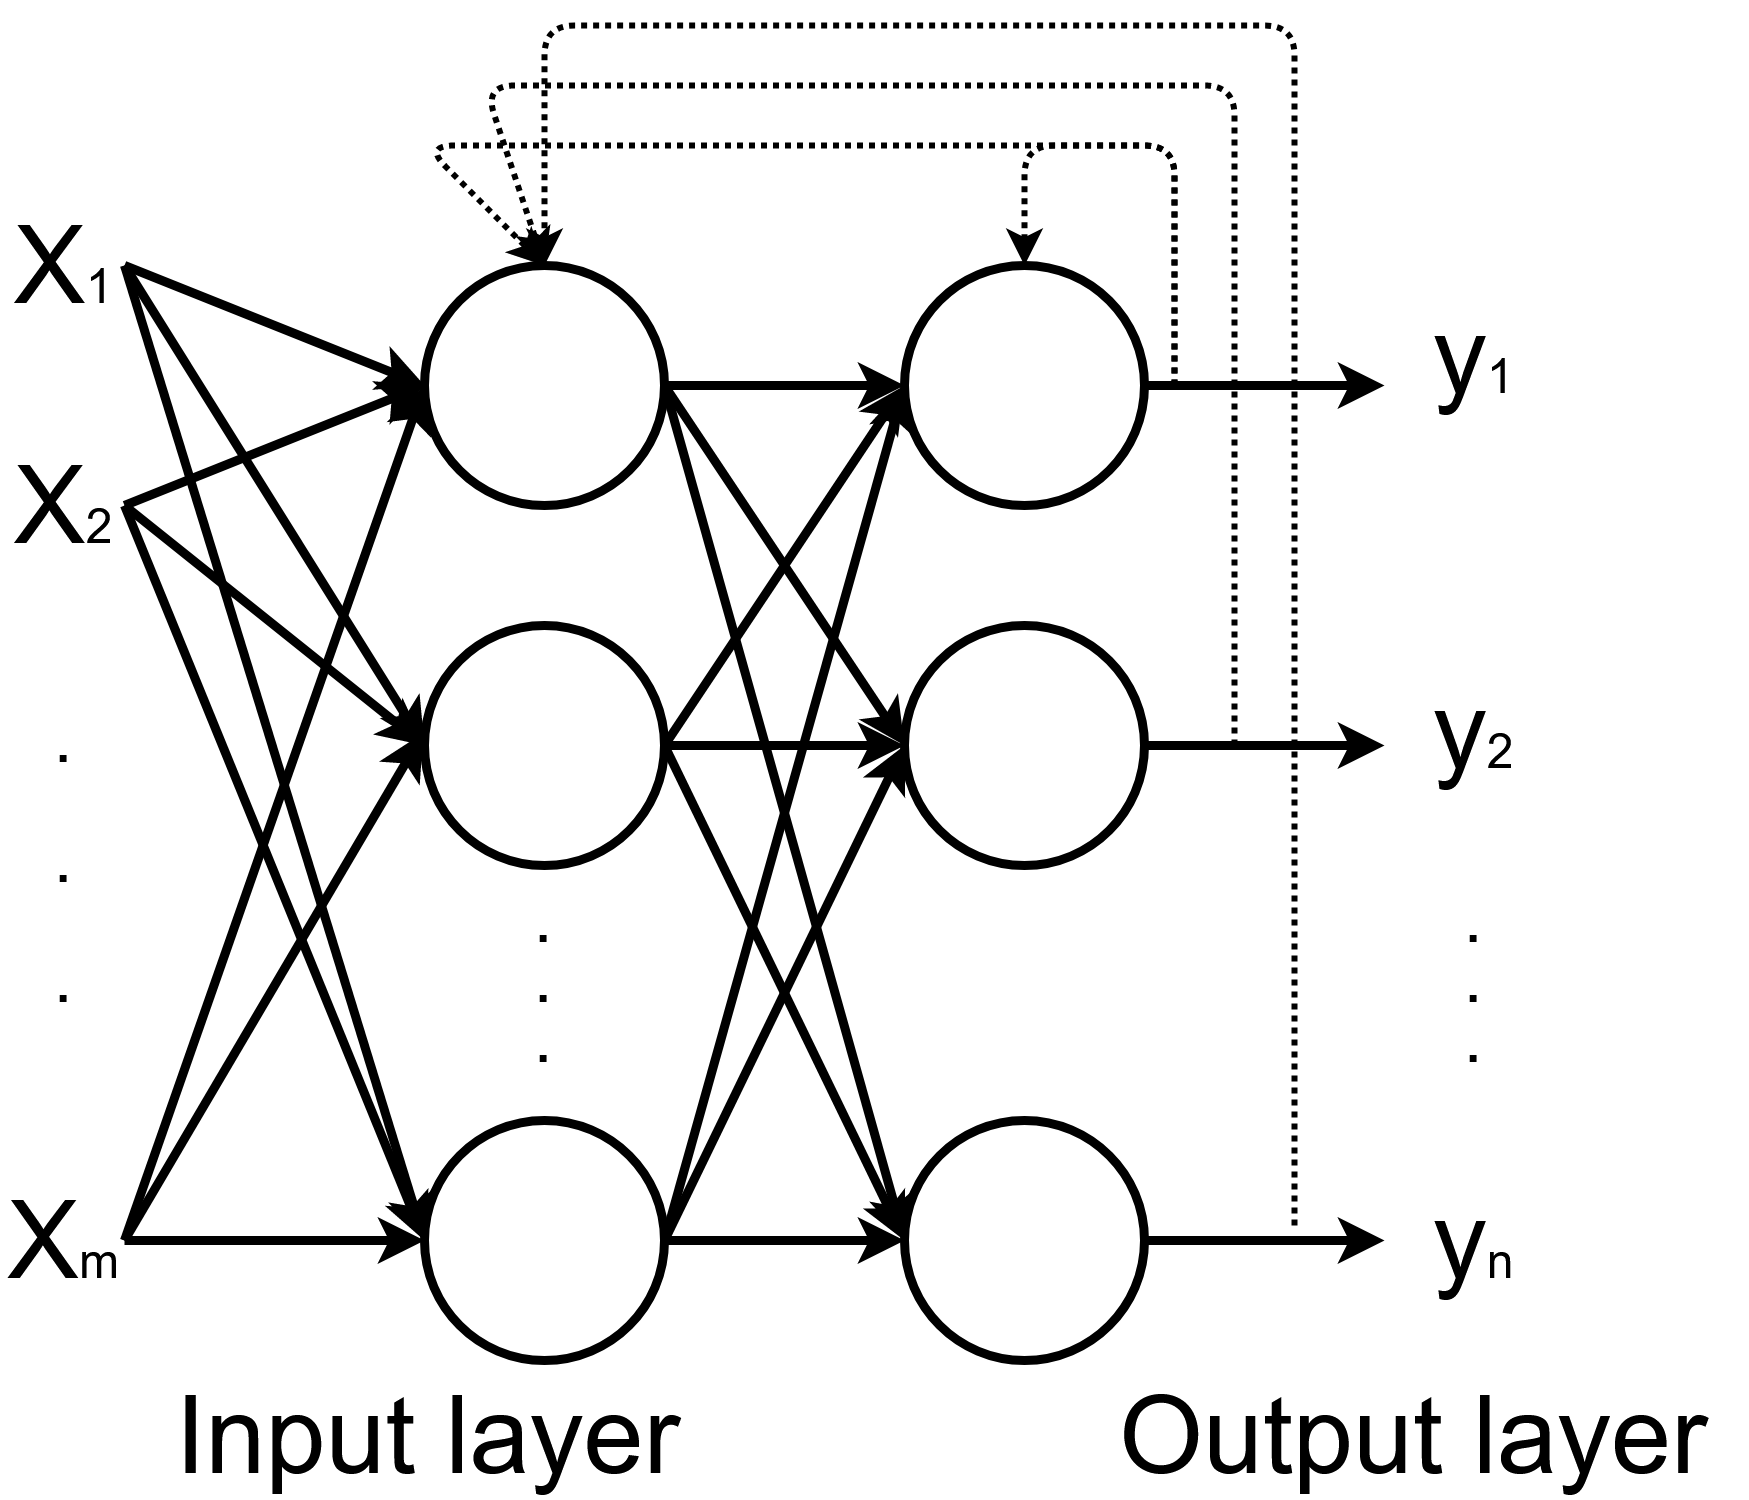
\includegraphics[width=0.49\textwidth]{Images/rnn.png}
    \caption{Structure of a Recurrent Neutral Network (RNN).}
    \label{rnn}
    \end{center}
\end{figure}



Backpropagation is also used in \ac{RNN}s and, although these models present a good behavior in temporal data prediction and modeling, it is difficult to train vanilla \ac{RNN}s whose data has a great temporal dependence. This is due to the gradient of the loss function that decays exponentially over time (which is referred to as the gradient vanishing problem)\cite{rnn4}. To tackle this problem, new types of \ac{RNN}s have been developed, such as \ac{LSTM}s and \ac{GRU}s, and whose behavior will be explained in a later chapter, whose architectures tend to mitigate this sort of issues, making them ideal for time series forecasting problems.

\subsection{Support vector machines (SVMs)}

Another very popular \ac{ML} methodology is the \ac{SVM}. Introduced by Cortes, Corinna and Vapnik in 1995 \cite{svm1}, \ac{SVM}s are widely applied to estimate the relationship between nonlinear inputs and real-value continuous outputs in time. \ac{SVR} is a specific type of \ac{SVM} used for regressions and it is an algorithm that allows the user to choose how tolerant he/she is with errors. The tolerance can be controlled both through an acceptable error margin ($\varepsilon$), or through tuning an acceptable error rate. The whole operation of a \ac{SVR} is based on the creation of a decision function $F(x_i)$, that is constructed by performing some training with historical data.

\begin{equation}
   F(x_i) = \langle w, \varphi(x_i) \rangle + b,
   \label{svmdec}
\end{equation}

where $\langle\cdot,\cdot\rangle$ represents the inner product, $w$ represents weight defined in $R^N$, $\varphi(x_i)$ represents the non-liner mapping of the input space to a high-dimensional feature space, and $b$ represents the bias\cite{svm2}. $w$ and $b$ are unknown variables, that are estimated by minimizing the regularized risk function \cite{svm2}. According to Magoules F. \cite{ann1}, the regularized risk can be solved using its dual form, by introducing the Lagrangian $L$

\begin{equation}
\begin{split}
       L & := \frac{1}{2}\parallel w \parallel^2 + c \sum_{i=1}^{n}(\xi_i + \xi_i^*) - \sum_{i=1}^{n}(\eta_i\xi_i + \eta_i^*\xi_i^*) - \sum_{i=1}^{n}a_i(\varepsilon + \xi_i - y_i- \langle w, \varphi(x_i) \rangle - b) \\ 
         & - \sum_{i=1}^{n}a_i^*(\varepsilon + \xi_i^* - y_i- \langle w, \varphi(x_i) \rangle - b),
\end{split}
\end{equation}

where $\{a_i, a_i^*, \eta_i, \eta_i^*\geq 0\}$ are the Lagrangian Multipliers, $\parallel w \parallel$ is the Euclidean norm, ${{\xi_i,\xi_i^*\geq 0}}$ are two slack variables to copy with some infeasible optimization constraints \cite{review2017}. Another constant $c \geq 0$ determines the trade-off between the training error (over-fitting) and model flatness (under-fitting) \cite{review2017}. 
It is important to mention that the Lagrange multipliers ($\eta_i = c - a_i$, $\eta_i^* = c-a_i^*$) are all independent. $\{a_i, a_i^*\}$ can be determined by the corresponding dual optimization \cite{ann1}:

\begin{equation}
\begin{split}
       & Maximize \  W(a_i, a_i^*) = -\frac{1}{2}\sum_{i=1}^{n}\sum_{j=1}^{n}(a_i-a_i^*)(a_j-a_j^*)(\varphi(x_i)\cdot \varphi(x_j) + \\
       & \sum_{j=1}^{n}(a_i-a_i^*)y_i - \varepsilon \sum_{j=1}^{n}(a_i+a_i^*),\\
       & subject \  to \begin{cases} \sum_{j=1}^{n}(a_i-a_i^*) = 0 \\ a_i, a_i^* \in [0,c] \end{cases} .
\end{split}
\end{equation}

After computing $a_i, a_i^*$, one can write $w$ as a function of $\{ a_i, a_i^*. x_i\}_{i=1}^n$. One can then infer the decision function for \ac{SVR}
\begin{equation}
      F(x) = \sum_{x_i \in SV} (a_i-a_i^*)K(x, x_i)+b , 
      \label{ioi}
\end{equation}
 where $K(x, x_i) = \varphi(x)\cdot\varphi(x_i)$. In \ac{ML}, one can call this function the \ac{SVR} kernel function, which varies according to the intended final application. Another aspect to consider is that the sum presented in the Equation \ref{ioi} does not include all the inputs, only the support vectors. Moreover, the bias $b$ is calculated based on these support vectors

\begin{equation}
\begin{split}
       b = & \frac{1}{N_1} \Bigg\{ \sum_{a_i \in (o,C)} \Bigg[ Y_i-\sum_{x_k\in SV}(a_j-a_j^*)K(x_i, x_j) - \varepsilon \Bigg] + \\
           & \sum_{a^*_j \in (o,C)}\Bigg[Y_i-\sum_{x_k\in SV}(a_j-a_j^*)K(x_i, x_j) - \varepsilon\Bigg] \Bigg\},
\end{split}
\end{equation}
 where $N_1$ is the number of support vectors. After the decision function, i.e., Equation \ref{svmdec}, is fully defined by the training process, the \ac{SVR} model created is ready to compute predictions for a new input \cite{review2017}.
 

\subsection{Statistical regression}

The third family of methods is the statistical regression family. This is a set of methods quite famous for their simplicity of use in the area of forecasting building consumption.This solution is based on the attempt to map a relationship between the outputs and the inputs that contribute to the behavior of the system. The statistical regression methodologies create a probabilistic model capable of relating different variables, which contribute to an output given by 
\begin{equation}
       Y_i = \alpha_i + \beta_1 x_{i,1} + \beta_2 x_{i,2} + ... + \beta_m x_{i,m} + \varepsilon_i,\quad if \  multiple,
\label{multi}
\end{equation}
or
\begin{equation}
       Y_i = \tilde{\alpha_i} + \tilde{\beta_1} x_{i,1} + \tilde{\beta_2} x_{i,2}^2 + ... + \tilde{\beta_m} x_{i,m}^m + \varepsilon_i,\quad if \  polynomial,
\label{poly}
\end{equation}

where $x_i$ represents the input, $\varepsilon_i$ represents a random normally distributed error, and  $\alpha_i, \tilde{\alpha_i}, \beta_j\  and\  \tilde{\beta_j}\ (j=1,...,m)$ are the parameters to be estimated. For instance, let's focus on multiple linear regression, Equation \ref{multi}, in which the estimates of all the parameters where computed using the \ac{LS} method. Let's also introduce the notion of \ac{SSE} as

\begin{equation}
       SSE = \sum_{i=1}^n (y_i-A_i-B_1 x_{i,1} - B_2 x_{i,2} - ... - B_m x_{i,m})_i^2,
\label{SSE}
\end{equation}
 where $A_i$ and $B_j(j\ =\ 1,...m)$ are the corresponding \ac{LS} estimates of $\alpha_i$, $\beta_j(j\ =\ 1,...m)$ in Equation \ref{multi} \cite{review2017}. Using this method, one should proceed to the minimization of the SSE that originates $m+1$ equations, in which each one of them presents a partial derivative of the \ac{SSE} in order to $A_i$ and $B_j(j=1,...,m)$ that should be equal to zero. It is through these equations that it is possible to determine the parameters $A_i$ and $B_j(j=1,...,m)$ that refer to the respective historical data. One can then write the equation
 
\begin{equation}
       y_i = A_i + B_1 x_{i,1} +  B_2 x_{i,2} + ... + B_m x_{i,m},
\label{y_i}
\end{equation}

known as the predictive equation with the estimated parameters in the form of multiple linear regression.
 
This model has become popular in forecasting medium to long term patterns, and is widely used for that purpose. As a down side, in order to make a good forecast, a large amount of data is needed, which makes this model limited by temporal constraints, that means that is not suitable when there is a small amount of time available to run the model. As far as short term forecasting is concerned, it has been found that it presents worse results than models such as \ac{ANN}s and \ac{SVM}s.

\subsection{Decision Trees (DT)}

\ac{DT} models \cite{dt1}, structurally present a tree inspired architecture consisting of a graph that has a root node and a set of branch nodes. In this architecture, the system inputs are inserted in the root node, where they are divided successively in different groups as they advance in the tree, based on a predetermined division criterion. The split data is then propagated to sub-nodes as branches from the root node. The inner nodes of the tree subsequently apply divisions of the sub-data into new sub-data. The end nodes, or leaf nodes, serve as output nodes. This type of methodologies can also be applied to the concrete case of energy forecasts of buildings. In the Figure \ref{dt} one can see an example where the range of consumption values is divided into hierarchical groups and the model classifies in the future the consumption of the building associating it with one of these groups.


\begin{figure}[h!]
    \centering
    \begin{center}
    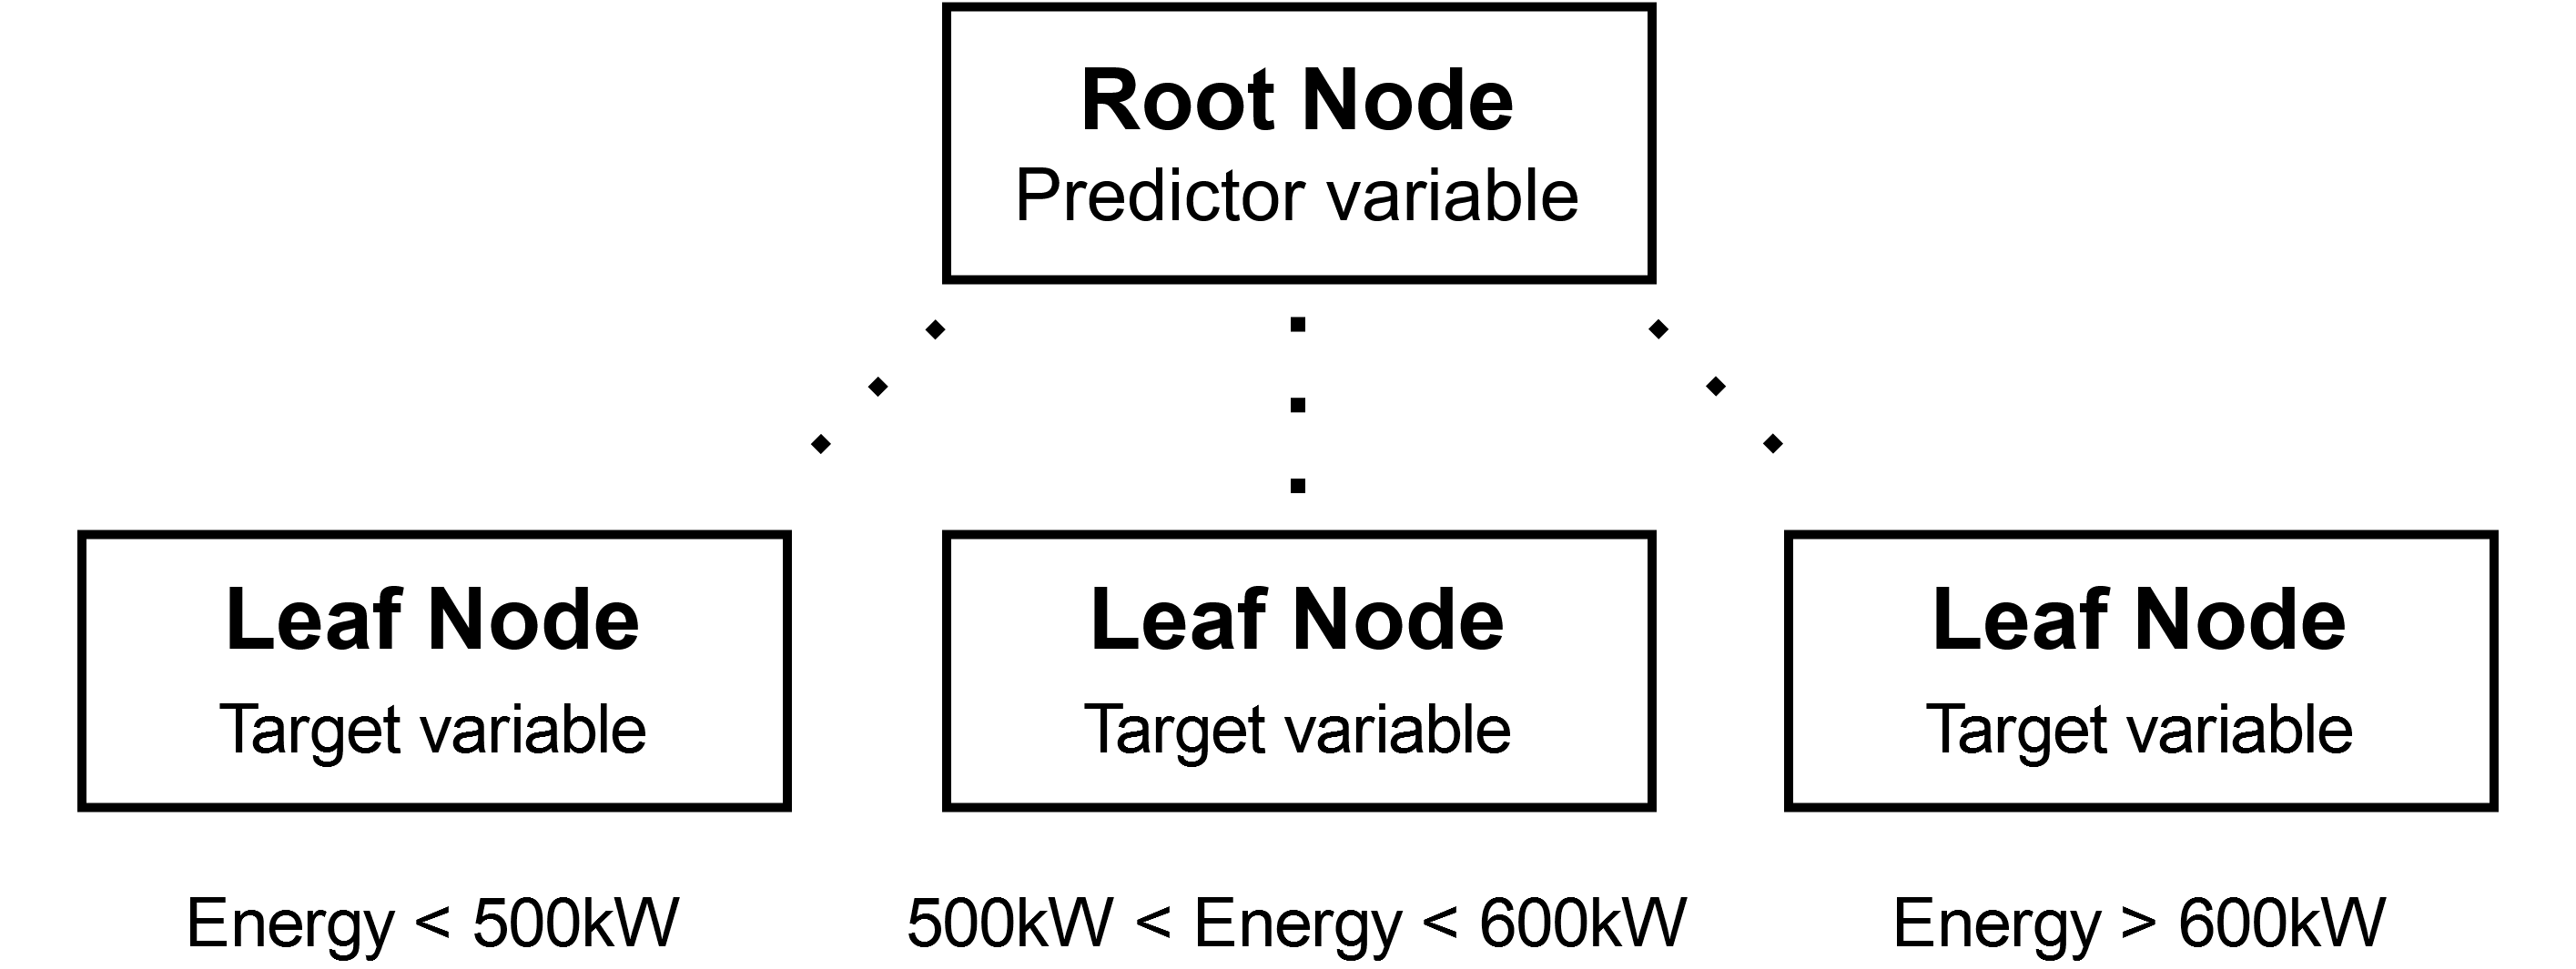
\includegraphics[width=0.6\textwidth]{Images/DT.png}
    \caption{Decision tree example.}
    \label{dt}
    \end{center}
\end{figure}

A relevant concept when it comes to the use of \ac{DT}s, is the concept of entropy
\begin{equation}
       E=\sum_{i=1}^n -P_i\log_2P_i,
\label{entropy}
\end{equation}

where $E$ is the information entropy, $n$ is the number of different target values and $P_i$ is the probability of a dataset taking the $i^{th}$ target value. This parameter is used to calculate the gain ratio of the \ac{DT}.

The major advantage of using this type of methodologies is the fact that it is a simple method to implement and does not require extensive computational knowledge to put it to work. Compared to other data-driven methods, the main disadvantage is that the targets or categories defined for leaf nodes are based on assumptions. In the example in Figure \ref{dt}, the previously defined energy ranges are the ones presented, because there is an expectation that the future values fit into one of the categories. This limitation can sometimes generate errors or deviations from the real values. The architecture of this model is also in itself a limitation because it does not present a good performance for nonlinear data \cite{dt2}.


\section{Data-driven prediction models applied to building energy forecasting \label{c}}

Both the architectural and the technical specifications of a building, such as the type of glass used, geographical position, etc., have determinant impact on the way this kind of structures manage their production and energy consumption. 

Electricity consumption has increased in the commercial sector in the last fifteen years.  In commercial buildings, annual energy consumption per square meter of floor space is over 200 kW h, with air conditioning being the final application that consumes the most energy within a building\cite{pie_1}. In Figure \ref{buildingenergy} \cite{pie_1}, a pie chart with the distribution of energy consumption in commercial buildings, in several groups, can be found.


\begin{figure}[h!]
    \centering
    \begin{center}
    \begin{tikzpicture}
    \pie[color={black!10, black!20, black!30, black!40}, text=pin]
        {4/Refrigeration, 
         4/Cooking,
         6/Lighting,
         7/Electronics,
         7/Others,
         9/Space cooling,
         18/Water heating,
         45/Space heating}
         
    \end{tikzpicture}
    \caption{End use wise energy consumption in commercial buildings.}
    \label{buildingenergy}
    \end{center}
\end{figure}


As can be seen in Figure \ref{buildingenergy}, space cooling, space heating and water heating represent  over 70\% of a building's energy consumption, which presents a direct correlation with  the number of people inside the building at each moment.

The ability to build models that take these factors into consideration and that can predict what the future energy consumption of the building will be, is a competence that enables not only the creation of sustainable solutions, but also the design of optimization models for managing these consumption sources, limiting their usage when unnecessary. According to Deb et al. \cite{reviewtsf}, factors such as occupancy schedule, weather conditions, thermal properties of building materials, complex interactions of the energy systems like \ac{HVAC} and lighting etc., have a high impact on the consumption behavior of a building. 

Taking into account all the necessary building specifications when applying white and grey-box techniques, it is quite complex to build a model capable of simulating the behavior of the building. In this sense, data-driven methods appear as a viable alternative. These techniques are based on past recorded data, and try to construct a future model based on past observed energy patterns. Techniques that use past data to develop a model to predict future behaviour, often fall under the category of \ac{ML}, and have been actively applied to building energy forecasting studies in the last two decades. Taking all into consideration, let's then look at some concrete cases where the models described above have been applied in forecasting energy consumption of buildings.

%The use of a simple prediction model has been common practice for many years, but with the progress of technology and computational capacity, the combination of several prediction models has become more and more common. In this regard, it is important to mention two very relevant model architectures, Ensemble models and Hybrid models. Ensemble models consist of models composed of several different machine learning techniques in parallel, where the different models work separately. Each of the models gets a certain answer, and then there is a voting system that determines the final forecast. Hybrid models are also composed of several different machine learning techniques, but which work in series, where the result obtained by a certain model is introduced as input to the next model. In this type of architecture the two models work together to obtain a single output (there is no voting). These two model typologies allow to obtain not only a better predictive performance than the one that would have been obtained using the models separately, but also more flexibility in model construction.

In Appendix B, Table \ref{table1}, the reader may find all the applications mentioned in this section, the type of building involved, the input data, the output data, the size of the dataset and the type of models used. According to Magoulès et al. \cite{ann1}, \ac{ANNs} are the most widely used artificial intelligence models in the application of building energy prediction. D. Datta et al. \cite{annr1} started, in 2000, to apply \ac{BPNN}s to forecast the energy consumption of a supermarket and since then, different \ac{BPNN}s models have been widely used in forecasting energy consumption of different types of buildings, such as office buildings, commercial buildings, residential buildings, etc. \cite{annr4}, \cite{annr9}, \cite{annr13}, \cite{annr14}, \cite{annr17} and \cite{annr19}. Kalogirou et al. \cite{annr2} also explores the integration of \ac{ANN}s for predicting the energy consumption of a building that has integrated solar panels by applying a combination of \ac{RNN}s with a \ac{BPNN} model to predict the energy consumption of a seasonal holiday house. Yang et al. \cite{annr3} predicted one day ahead electric consumption of an office building by experimenting a sliding window \ac{ANN} methodology and accumulative \ac{ANN} methodology. Both Yezioro et al. \cite{annr5}, and Yokoyama et al. \cite{annr7}, developed systems to forecast more specific indicators, both heating and cooling energy consumption of a building, by using \ac{BPNN}s, as well as Ekici et al. \cite{annr6}, just for heating and Cheng-wen et al. \cite{annr8}, just for cooling. Later another methodology for forecasting energy consumption of buildings was also tested, which applies a \ac{BPNN} with multiple outputs \cite{annr10} so that one could choose the best option from the results obtained, and Li et al.\cite{annr12} proposed two hybrid models, the \ac{iPSO-ANN} which adjusts the weights of the neural network, and the \ac{GA-ANN} model.
On the other hand, Deb et al. \cite{annr15}, Shi et al. \cite{annr16}, Hossen et al. \cite{annr18} and Gasparin et al. \cite{annr21},  have also used \ac{RNN}s to predict energy consumption of both office and residential buildings, and have concluded that this type of models present high accuracy, based on the use and knowledge of past consumption data of the buildings in question. Ruiz et al. \cite{annr22} introduced a methodology to predict future energy consumption using \ac{NAR} and the \ac{NARX}, respectively.
Finally, Deb et al. \cite{annr20}, used \ac{BPNN}s to create energy saving systems associated with the use of \ac{HVAC} in office buildings.
Li et al. \cite{annr24} developed a new hybrid method called \ac{TLBO-ANN}, to optimize \ac{ANN}’s parameters in order to forecast two actual building consumptions. Ruiz et al. \cite{annr25} was also able to predict the energy consumption of multiple university buildings by applying Elman neural networks with evolutive optimization in 2018. Fan et al. \cite{annr26} compared \ac{LSTM}s and \ac{GRU}s, while predicting the energy consumption of an educational building and He et al. \cite{annr27}, Wua et al. \cite{annr28} and Kim et al. \cite{annr29} developed examples of hybrid models combining several types of \ac{ANN}s with the same purpose. 


In 2005, Dong et al. \cite{svm2} applied \ac{SVM}s to predict the energy consumption of a commercial building in a tropical region. Then, in 2009, Li et al. \cite{svmr1} also applied \ac{SVM}s to predict the hourly cooling load of a building. Later, in 2010, Paudel et al. \cite{svm3} implemented an architecture with two parallel \ac{SVM}s to predict heating demand and electrical load of several office buildings and in 2017, et al. \cite{svmr7}, used again \ac{SVM}s to predict the consumption of a residential building. In 2010 Xuemei et al. \cite{svmr2}, introduced a \ac{FSVM} and fuzzy c-mean clustering for predicting the cooling load of Zhongkai university scientific building, and concluded that \ac{FSVM} has better effectiveness and efficiency in the learning and prediction in contrast to others, such as classical \ac{SVM}s. Edwards et al. \cite{svmr3} developed a case study where he implemented a \ac{SVR} to predict hourly electrical consumption of a residential building, and Zhang et al. \cite{svmr4} combined also \ac{SVR}s with a differential evolution optimization technique for the same purpose. Ma also et al. \cite{svmr5} also applied \ac{SVM}s to tackle the same problem in China, and concluded that \ac{SVM} model forecasts are well aligned with the statistic values in all the seven zones of the country tested, as well as with the whole nation's data. Lastly, in 2019, Zhong et al. \cite{svmr6}, also applied \ac{SVR}s for building energy consumption prediction of an office building and concluded that "The energy consumption prediction obtained by applying the proposed models to a real office building can provide an accurate energy consumption scheduling plan for the power system, which has practical significance for energy planning, management, and conservation". \ac{SVM}s are models that can obtain good results for forecasting building's energy profiles because they can deal with non-linear relations by transforming them into linear relations in a higher dimension. On the other hand, Zhao et al. \cite{svm3}, Dong et al. \cite{svm2} and Li et al. \cite{svm5}, identified that \ac{SVM} is a slow model for large scale problems.
 
In 2015 Fumo et al. \cite{regression0} applied both simple and multiple regression analysis in a case study regarding residential buildings. Later in 2018, Ahmad et al. \cite{dt0} applied both DTs and regression models for predicting the consumption behaviour of multiple buildings.

There are also studies that evaluate different models by applying them to the same case study. In 2009, et al. \cite{svmr0}, Setiawan compared several methods when performing load forecasting, and concluded that the \ac{SVR} model could outperform the \ac{BPNN}s, but simpler models such as linear regression could produce similar accuracy results in a much faster way. Seyedzadeh et al. \cite{other2}, also tested different models for predicting energy consumption of buildings and concluded that \ac{GBRT} provide the most accurate predictions. However, when the data was simple (in terms of input variables and size), \ac{SVM} was proven to be the best choice because of simplicity and the speed of calculations. Lastly, Fan et al. \cite{other1}, compared the results when manipulating the features of a \ac{GAN}, which helped to bridge the knowledge gap between deep learning and building operations. 

Besides the models presented, there are also other data-driven models that were applied with the same purpose. Although not used so regularly, less common models have been gaining some relevance in recent years, namely due to the significant increase in computing available power. Most of these methods are also a sub-category of the methods presented above. \ac{ANFIS}, is a model that has an architecture similar to an artificial neural network, developed in the early 1990s by Jang et al. \cite{anfis1}, \cite{anfis2}. This methodology complements \ac{ANN}s with fuzzy logic principles \cite{anfis3}, which allows defining if-then rules to approximate non-linear functions that led Jang et al. \cite{anfis4} to classify \ac{ANFIS} as an universal estimator. Wang et al. \cite{rf0} used a \ac{RF} technique, compared it to the most common approaches such as \ac{SVM}s and tried to demonstrate that RF is also a good choice when trying to predict building energy consumption. Other method, \ac{ELM}, consists of feed-forward neural networks where the parameters of the hidden nodes don't need to be tuned. These hidden nodes can be randomly assigned, or can be inherited from their ancestors without being changed. Usually, the output weights of the hidden nodes are learned in a single step, which resembles the linear learning process. According to Guang-Bin Huang \cite{elm1}, the advantage of these models is their capability of producing a good generalization performance and learn in a faster pace than networks trained using back-propagation, and according to Huang et al. \cite{elm2}, \cite{elm3} and \cite{elm4}, these models have the capability to outperform support vector machines in both classification and regression applications.

The use of a simple prediction model has been a common practice for many years, but with the progress of technology and computational capacity, the combination of several prediction models has become more and more common. In this regard, it is important to mention two very relevant model architectures: Ensemble architectures and Hybrid architectures. Ensemble architectures consist of models composed by several different machine learning techniques in parallel, where the different models work separately. Each of the models gets a certain answer, and then there is a voting system that determines the final forecast. Hybrid architectures are also composed of several different machine learning techniques working in series, where the result obtained by a certain model is introduced as input to the next model. In this type of architecture the two models work together to obtain a single output (there is no voting). These two model architectures allow to obtain not only a better predictive performance than the one that would have been obtained using the models separately, but also more flexibility in model construction.


\section{Conclusion}

In this section we introduced the main topics related to power availability forecast and the work done in this area. In the section \ref{a}, we started by doing a brief introduction of the different types of predictive methodologies and we explained the difference between each of them. Then, in section \ref{b}, we have distinguished the different data-driven models and introduced theoretically the most common models in this branch. Lastly, in the section \ref{c} we presented some of the most important applications of data-driven models for forecasting energy consumption of buildings, specifically.
